% !TEX TS-program = XeLaTeX
% use the following command:
% all document files must be coded in UTF-8
\documentclass[portuguese]{textolivre}
% build HTML with: make4ht -e build.lua -c textolivre.cfg -x -u article "fn-in,svg,pic-align"

\journalname{Texto Livre}
\thevolume{15}
%\thenumber{1} % old template
\theyear{2022}
\receiveddate{\DTMdisplaydate{2022}{1}{06}{-1}} % YYYY MM DD
\accepteddate{\DTMdisplaydate{2022}{3}{28}{-1}}
\publisheddate{\DTMdisplaydate{2022}{4}{19}{-1}}
\corrauthor{Teresa Ribeirinha}
\articledoi{10.35699/1983-3652.2022.37789}
%\articleid{NNNN} % if the article ID is not the last 5 numbers of its DOI, provide it using \articleid{} commmand 
% list of available sesscions in the journal: articles, dossier, reports, essays, reviews, interviews, editorial
\articlesessionname{articles}
\runningauthor{Ribeirinha et al.} 
%\editorname{Leonardo Araújo} % old template
\sectioneditorname{Daniervelin Pereira}
\layouteditorname{Leonado Araújo}

\title{O envolvimento cognitivo e o desempenho acadêmico do aluno do ensino secundário no modelo \textit{Flipped Classroom} na educação a distância}
\othertitle{Cognitive engagement and academic performance of secondary school students on the Flipped Classroom model in distance education}
% if there is a third language title, add here:
%\othertitle{Artikelvorlage zur Einreichung beim Texto Livre Journal}

\author[1]{Teresa Ribeirinha \orcid{0000-0002-5678-3476} \thanks{Email: \url{teresaribeirinha@hotmail.com}}}
\author[1]{Bento Silva Duarte \orcid{0000-0001-5394-5620} \thanks{Email: \url{bento@ie.uminho.pt}}}
\author[2]{Paulo Ribeirinha \orcid{0000-0003-0191-4317} \thanks{Email: \url{paribeirinha@fe.up.pt}}}
\author[3]{Regina Alves \orcid{0000-0001-7189-5487} \thanks{Email: \url{rgnalves@gmail.com}}}
\affil[1]{Universidade do Minho, Instituto de Educação, Centro de Investigação em Educação, Braga, Portugal.}
\affil[2]{Universidade do Porto, Faculdade de Engenharia, Porto, Portugal.}
\affil[3]{Universidade do Minho, Instituto de Educação, Centro de Investigação em Estudos da Criança, Braga, Portugal.}

\addbibresource{article.bib}
% use biber instead of bibtex
% $ biber article

% used to create dummy text for the template file
\definecolor{dark-gray}{gray}{0.35} % color used to display dummy texts
\usepackage{lipsum}
\SetLipsumParListSurrounders{\colorlet{oldcolor}{.}\color{dark-gray}}{\color{oldcolor}}

% used here only to provide the XeLaTeX and BibTeX logos
\usepackage{hologo}

% if you use multirows in a table, include the multirow package
\usepackage{multirow}

% provides sidewaysfigure environment
\usepackage{rotating}

% CUSTOM EPIGRAPH - BEGIN 
%%% https://tex.stackexchange.com/questions/193178/specific-epigraph-style
\usepackage{epigraph}
\renewcommand\textflush{flushright}
\makeatletter
\newlength\epitextskip
\pretocmd{\@epitext}{\em}{}{}
\apptocmd{\@epitext}{\em}{}{}
\patchcmd{\epigraph}{\@epitext{#1}\\}{\@epitext{#1}\\[\epitextskip]}{}{}
\makeatother
\setlength\epigraphrule{0pt}
\setlength\epitextskip{0.5ex}
\setlength\epigraphwidth{.7\textwidth}
% CUSTOM EPIGRAPH - END

% LANGUAGE - BEGIN
% ARABIC
% for languages that use special fonts, you must provide the typeface that will be used
% \setotherlanguage{arabic}
% \newfontfamily\arabicfont[Script=Arabic]{Amiri}
% \newfontfamily\arabicfontsf[Script=Arabic]{Amiri}
% \newfontfamily\arabicfonttt[Script=Arabic]{Amiri}
%
% in the article, to add arabic text use: \textlang{arabic}{ ... }
%
% RUSSIAN
% for russian text we also need to define fonts with support for Cyrillic script
% \usepackage{fontspec}
% \setotherlanguage{russian}
% \newfontfamily\cyrillicfont{Times New Roman}
% \newfontfamily\cyrillicfontsf{Times New Roman}[Script=Cyrillic]
% \newfontfamily\cyrillicfonttt{Times New Roman}[Script=Cyrillic]
%
% in the text use \begin{russian} ... \end{russian}
% LANGUAGE - END

% EMOJIS - BEGIN
% to use emoticons in your manuscript
% https://stackoverflow.com/questions/190145/how-to-insert-emoticons-in-latex/57076064
% using font Symbola, which has full support
% the font may be downloaded at:
% https://dn-works.com/ufas/
% add to preamble:
% \newfontfamily\Symbola{Symbola}
% in the text use:
% {\Symbola }
% EMOJIS - END

% LABEL REFERENCE TO DESCRIPTIVE LIST - BEGIN
% reference itens in a descriptive list using their labels instead of numbers
% insert the code below in the preambule:
%\makeatletter
%\let\orgdescriptionlabel\descriptionlabel
%\renewcommand*{\descriptionlabel}[1]{%
%  \let\orglabel\label
%  \let\label\@gobble
%  \phantomsection
%  \edef\@currentlabel{#1\unskip}%
%  \let\label\orglabel
%  \orgdescriptionlabel{#1}%
%}
%\makeatother
%
% in your document, use as illustraded here:
%\begin{description}
%  \item[first\label{itm1}] this is only an example;
%  % ...  add more items
%\end{description}
% LABEL REFERENCE TO DESCRIPTIVE LIST - END


% add line numbers for submission
%\usepackage{lineno}
%\linenumbers

\begin{document}
\maketitle

\begin{polyabstract}
\begin{abstract}
O envolvimento cognitivo (EC) do aluno é um pré-requisito para uma aprendizagem significativa. Este texto analisa o EC do aluno numa proposta baseada no modelo \textit{Flipped Classroom} (FC) na educação a distância (EaD). Implementou-se a proposta no ensino secundário português, através de um ciclo de investigação-ação, durante a pandemia Covid-19, com aulas assíncronas e síncronas divididas em atividades conduzidas pelo professor (ACP) e atividades centradas no aluno (ACA). Com o objetivo de compreender a influência do design das atividades no EC do aluno e o impacto da proposta nos desempenhos acadêmicos dos alunos, analisaram-se os discursos dos alunos, as percepções sobre a EaD e os testes de avaliação de conhecimentos. Os resultados mostraram níveis superiores de EC do aluno nas ACA, pois estas permitiram um papel mais ativo dos alunos na construção do conhecimento, uma maior facilitação da professora e aprendizagens com os pares. Os desempenhos acadêmicos dos alunos foram superiores na EaD comparativamente ao ensino presencial, o que pode estar associado aos indicadores de EC (\textit{autopercepções positivas, autoeficácia e compreensão dos conteúdos}) identificados nas percepções dos alunos. Porém, a mesma análise também identificou vários aspetos que carecem de melhoria para potenciar o modelo FC na EaD.

\keywords{Sala de Aula \textit{on-line} \sep Educação a distância \sep Estudantes \sep Envolvimento cognitivo}
\end{abstract}

\begin{english}
\begin{abstract}
Cognitive engagement (CE) is a prerequisite for students’ meaningful learning. The present text analyses the student's CE in a proposal based on the Flipped Classroom (FC) model, in distance education (DE). The proposal was implemented through an action-research cycle in Portuguese secondary schools during the Covid-19 pandemic. It combined asynchronous and synchronous lessons divided into teacher-led activities (TLA) and student-centred activities (SCA). To understand the influence of the design of the activities in the student's CE and the impact of the proposal on the students' academic performances, the students' discourses, perceptions, and knowledge assessment tests were analysed. The results showed higher levels of student CE in ACA, as it allowed for a more active role for the students in knowledge construction, greater facilitation from the teacher and peer learning. The results of the students' academic performance were higher in DE than in face-to-face teaching. This may be associated with the CE indicators (positive self-perceptions, self-efficacy, and content understanding) identified in the students' perceptions. However, the same analysis also identified several aspects that need improvement to enhance the FC model in DE.

\keywords{Online classroom \sep Distance Education \sep Students \sep Cognitive engagement}
\end{abstract}
\end{english}
% if there is another abstract, insert it here using the same scheme
\end{polyabstract}

\section{Introdução}\label{sec-intro}
Em Portugal, a pandemia causada pela Covid-19 (SARS-Cov-2) forçou, por duas vezes, a transição de todo o processo de ensino-aprendizagem para a modalidade digital para dar continuidade à formação dos alunos. Porém, se da primeira vez foi implementado um ensino remoto emergencial, por carecer de planejamento e de formação adequada dos professores \cite{bozkurt_emergency_2020}; da segunda vez, supostamente ajustadas as condições de implementação, as instituições escolares chamaram-lhe de Educação a Distância (EaD). 

Na conceitualização dessa modalidade, além da separação física de professores e alunos, existem outras caraterísticas determinantes, nomeadamente, a interação entre os participantes através de ferramentas de comunicação síncronas e assíncronas, o estudo autônomo dos alunos e a existência de apoio institucional \cite{espino-diaz_creating_2020}. Todavia, são vários os fatores que contribuem para o tempo que os alunos são capazes de se comprometer com as tarefas e para a eficácia dos seus esforços. Assim, se por um lado, os alunos valorizam o ambiente criado pela quantidade significativa de interação gerada nas plataformas de aprendizagem \textit{e-learning} e as oportunidades de compartilhar ideias e recursos com pares \cite{espino-diaz_creating_2020}; por outro, distraem-se mais facilmente e apresentam dificuldades em se autorregularem \cite{xu_effects_2020}. 

Nesse sentido, o envolvimento do aluno tem sido identificado consistentemente como um fator crítico para o seu sucesso acadêmico na EaD \cite{hampton_student_2016}. Surge positivamente relacionado com importantes resultados educacionais, como a satisfação, persistência e desempenhos acadêmicos dos alunos \cite{kuh_what_2009} e, embora seja amplamente investigado, não há consenso acerca da sua definição exata e composição \cite{eccles_engagement:_2016}.

Neste estudo\footnote{Este estudo foi aprovado pela Comissão de Ética para a Investigação em Ciências Sociais e Humanas do Conselho de Ética da Universidade do Minho, com o código CEICSH 107/2019}, adotou-se a definição de envolvimento do aluno proposta por \textcite{bond_facilitating_2019}, que o descreve como a energia e o esforço que os alunos usam dentro da sua comunidade de aprendizagem, observável através de comportamentos, indicadores cognitivos e afetivos, sendo moldado por um conjunto de influências estruturais e internas, incluindo a interação complexa dos relacionamentos, atividades e ambiente de aprendizagem. Essa opção é justificada por dois argumentos: (1) está alinhada com as pesquisas que amplamente aceitam a existência de três dimensões do envolvimento do aluno \cite{fredricks_school_2004}: cognitiva (investimento psicológico dos alunos nas tarefas e o modo como usam estratégias autorreguladoras e metacognitivas para compreender e dominar conhecimentos), afetiva (respostas emocionais dos alunos ou sentimentos em relação aos professores, aos colegas, à aprendizagem e à escola) e comportamental (participação dos alunos numa atividade de aprendizagem, como completar uma tarefa, assistir às aulas ou contribuir nas discussões); (2) entende os resultados da atividade formativa como uma construção coletiva e sistêmica assente numa complexa estrutura mediadora \cite{engestrom_expansive_2001}.

Um aspeto determinante para o envolvimento do aluno no contexto \textit{on-line}, que decorre da própria conceitualização da modalidade de EaD, relaciona-se com o apoio institucional configurado nos esforços pedagógicos do professor. Este deve ser capaz de conceber um \textit{design} estratégico dos conteúdos a disponibilizar, suportado por diversos canais de interação com os seus alunos \cite{stone_online_2019}. Nesse sentido, os educadores que procuram maneiras de aumentar o envolvimento do aluno têm na modalidade híbrida uma possibilidade \cite{halverson_learner_2019}, dadas as evidências do potencial da tecnologia para aumentar a autoeficácia, autorregulação e participação dentro da comunidade educacional \cite{alioon_effect_2019}. 

O modelo \textit{Flipped Classroom} (FC) apresenta-se como um modelo de aprendizagem híbrida amplamente adotado porque responde à procura por ambientes de aprendizagem aprimorados pela tecnologia e centrados no aluno \cite{lai_multilevel_2021}. 

A implementação bem-sucedida do modelo, segundo a \textcite{flipped_learning_network_fln_four_2014}, deve atender a quatro pilares fundamentais definidos pela sigla F-L-I-P. Assim, a letra F (\textit{Flexible environment}) refere-se à criação de espaços que possibilitem aos alunos escolher onde e como aprender, trata-se de flexibilizar não só a sequência de aprendizagem, com a utilização de materiais diversos, mas também a avaliação. Esta flexibilização permite que o aluno, ao seu próprio ritmo, explore o material divulgado, assumindo assim o controle da sua aprendizagem, o que traduz a \textit{Learning culture} (L). Ao centrar o processo de aprendizagem no aluno, o professor assume a gestão e a orientação de todo o processo, através da seleção e criação de conteúdos relevantes para apoiar a aprendizagem dos alunos, \textit{Intentional Content} (I). O último pilar define o papel do professor, \textit{Professional Educator} (P), com capacidades de criar um ambiente de aprendizagem flexível, conduzir regularmente avaliações formativas, fornecer \textit{feedback} e refletir sobre a sua prática de modo a melhorá-la.

Neste estudo, implementou-se o modelo FC na EaD seguindo as diretrizes do FNL conjugando aulas assíncronas (ASS) com aulas síncronas (AS), dadas as evidências do sucesso do modelo nesse contexto de aprendizagem \cite{ribeirinha_flipped_2021}. A principal vantagem do modelo são as interações com os pares e professor desenvolvidas em contexto de aula, influenciando o modo como os alunos se envolvem nas tarefas, o que, por sua vez, afeta o nível de compreensão dos conteúdos, com repercussão nos resultados alcançados \cite{van_alten_effects_2019}. 

Assim, o sucesso do modelo está fortemente dependente do envolvimento do aluno, sendo, especificamente, o Envolvimento Cognitivo (EC) um pré-requisito para uma aprendizagem significativa \cite{solis_teaching_2008}, pois quando os alunos se envolvem cognitivamente com as tarefas são capazes de criar conhecimentos e alcançar maior compreensão nas discussões \textit{on-line} \cite{zhu_interaction_2006}. Uma forma de avaliar a qualidade da aprendizagem \textit{on-line} é avaliar o nível de EC dos alunos, pois esse é um indicador de que o processo de aprendizagem está a ocorrer, na medida em que os alunos exercem um esforço mental para se envolverem com os conteúdos \cite{shukor_predictive_2014}. 

Estudos sobre o modelo FC e o EC do aluno revelam resultados pouco consistentes \cite{bond_facilitating_2020}. Numa revisão sistemática de 107 estudos, no ensino k-12, \textcite{bond_facilitating_2020} indica que, em um quarto dos estudos analisados, o modelo FC potenciou os indicadores de EC do aluno, \textit{autopercepções positivas} e \textit{autoeficácia}, sendo a \textit{compreensão dos conteúdos}, também, bastante frequente. Porém, os indicadores \textit{relutância} e \textit{confusão} são igualmente prevalentes, pois alguns estudos relatam a dificuldade dos alunos em aceitar o modelo FC, uma vez que não estão dispostos a completar as tarefas de pré-aprendizagem e os vídeos, por vezes, geram mal-entendidos que prevalecem pelo fato de não serem imediatamente esclarecidos pelo professor. 

Sendo que a maioria dos estudos sobre o envolvimento do aluno usa métodos quantitativos \cite{bond_facilitating_2020} privilegiando as percepções dos alunos obtidas por questionário \cite{xu_effects_2020} e sendo a dimensão comportamental a mais frequentemente medida \cite{henrie_measuring_2015}, esta pesquisa tenta colmatar as falhas apresentadas na literatura ao explorar múltiplos recursos para compreender o modo como o EC do aluno se desenvolve em ambientes de EaD e qual a sua repercussão nos desempenhos acadêmicos dos alunos. Assim, investigou-se o EC do aluno a partir da análise dos seus discursos produzidos nas AS, complementando-se essa análise com as suas percepções sobre a experiência na EaD obtidas por entrevista. Posteriormente, aferiu-se o nível de compreensão dos conteúdos através dos desempenhos acadêmicos dos alunos obtidos em testes de avaliação de conhecimentos.

Esta pesquisa é suportada pela terceira geração da Teoria da Atividade (TA) de \textcite{engestrom_expansive_2001}, uma lente útil para estudar a aprendizagem intersubjetiva na EaD e cujos pressupostos estão em consonância com as ideias de construtivismo, aprendizagem situada e cognição distribuída e quotidiana \cite{bower_quantitative_2010}. Ao representar a atividade (formativa) como uma construção coletiva, \textcite{engestrom_expansive_2001} identifica seis elementos: o sujeito (indivíduo ou subgrupo), objeto (espaço do problema para o qual a atividade é direcionada), artefatos mediadores (ferramentas físicas ou simbólicas), comunidade (indivíduos ou subgrupos que partilham o mesmo objetivo), divisão do trabalho (divisão horizontal de tarefas entre membros de uma comunidade, bem como a divisão vertical de poder) e as regras (regulamentos implícitos e explícitos que restringem as interações no interior do sistema de atividade). Os sistemas de atividade usados nesta pesquisa estão representados na \Cref{fig01}.

\begin{figure}[htbp]
 \centering
 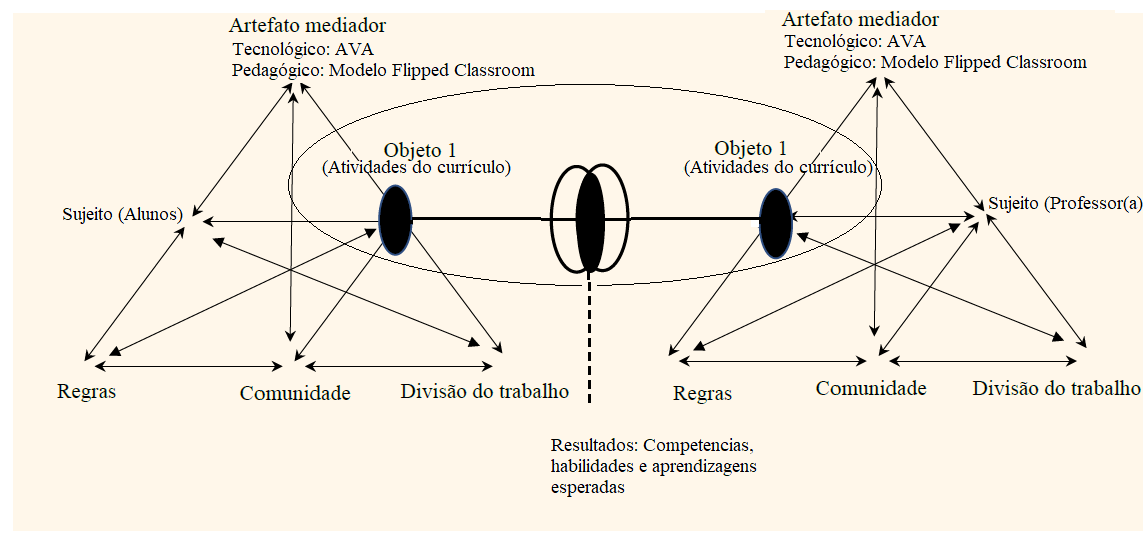
\includegraphics[width=0.85\textwidth]{fig1.png}
 \caption{Sistemas de atividade de alunos e professora para o modelo FC em contexto online.}
 \label{fig01}
 \source{Adaptado de \textcite{engestrom_expansive_2001}.}
\end{figure}

Na base desta teoria estão cinco princípios \cite{engestrom_expansive_2001}: (1) a existência de um \textit{sistema de atividade coletivo} em relação interativa, por orientar para um objeto coletivo mediado por artefatos que moldam e transformam o objeto em resultados; (2) a \textit{multivocalidade}, por considerar que os indivíduos que o integram possuem múltiplos pontos de vista, interesses e experiências; (3) a \textit{historicidade}, por admitir a transformação contínua dos sistemas de atividade ao longo do tempo; (4) as \textit{contradições}, por serem tensões estruturais acumuladas dentro e entre os sistemas que proporcionam oportunidades de mudanças e desenvolvimento do sistema de atividade; (5) a \textit{transformação expansiva}, por surgir em resposta às contradições que são alterações qualitativas que levam à reconfiguração do objeto e à transformação da prática educativa.

Assim, ao se utilizar como unidade de análise dois sistemas de atividade (professora e alunos), orientados para um objeto coletivo (atividades do currículo) e mediados, tecnologicamente, pelo ambiente virtual de aprendizagem (AVA) e, pedagogicamente, pelo modelo FC, pretende-se estudar os resultados dessa interação, nomeadamente o EC do aluno, o nível de compreensão dos conteúdos e as possíveis tensões que resultem dessa interação.

\section{Metodologia}\label{sec-normas}
Este estudo tem subjacente a experimentação de novas estratégias de ensino com o objetivo de adequar as práticas escolares às necessidades impostas pelo novo contexto \cite{maximo-esteves_visao_2008}. Assenta, portanto, em pressupostos da metodologia de Investigação-Ação (IA). Essa forma de investigação, efetuada pelos próprios participantes, de cariz autorreflexivo e induzida pela necessidade de compreensão e mudança de certas práticas educacionais, dá voz a todos os intervenientes, num processo colaborativo, que os capacita para o desenvolvimento dessas mudanças \cite{coutinho_investigacao-accao_2009}. Além disso, apresenta sobreposições com os princípios da TA e permite a incorporação de várias técnicas de recolha de evidências que imprimem robustez ao estudo realizado \cite{coutinho_investigacao-accao_2009}.

\subsection{Participantes e contexto de estudo}\label{sec-conduta}
A pesquisa decorreu numa turma de 11.º ano, do ensino secundário português, na disciplina de Física e Química (F.Q.), no período compreendido entre fevereiro e abril de 2021, que correspondeu ao período de EaD devido à pandemia COVID-19.   

A turma é composta por 23 alunos (14 alunos do sexo feminino, 9 do sexo masculino) e a média de idades é de 16,25 anos. O consentimento para a realização da pesquisa foi concedido por todos os participantes através do termo de consentimento informado.

A proposta pedagógica assente no modelo FC apresentava duas componentes: as Aulas Assíncronas (ASS) e as Aulas Síncronas (AS) divididas em dois momentos de aprendizagem. Essa divisão relaciona-se com o \textit{design} de atividades em \textit{e-learning} proposto por \textcite{clark_multimedia_2005} em: (1) Atividades Conduzidas pelo Professor (ACP): quando são transmitidos pequenos segmentos de informação, que podem ser exemplos ou demonstrações, intercalados com atividades realizadas pelos alunos sobre essa mesma informação, essa abordagem caracteriza-se pela existência de interação e \textit{feedback} professor-aluno; (2) Atividades Centradas no Aluno (ACA): quando os alunos realizam tarefas orientadas por objetivos e o fluxo discursivo entre os alunos permite a construção de conceitos formais através de uma aprendizagem colaborativa. O professor adota um papel de mediador.

Assim, nas ASS usava-se a plataforma de \textit{e-learning} \textit{Edmodo}, na qual os alunos exploravam os materiais disponibilizados pela professora, e que eram, normalmente, vídeos didáticos acompanhados por um \textit{quiz} de monotorização. Nas AS usava-se a plataforma \textit{Zoom}, nas quais o primeiro momento correspondia às ACP e na presença de todos os alunos eram debatidos os conteúdos das ASS, nomeadamente, os conteúdos do vídeo, as eventuais dúvidas e as respostas do \textit{quiz}. O segundo momento de aprendizagem correspondia às ACA, sendo os alunos distribuídos, aleatoriamente, por salas virtuais para em grupo realizarem um conjunto de atividades que incluíam resolução de problemas, exploração de simulações e análise de resultados experimentais.

\subsection{Recolha e tratamento de dados}\label{sec-fmt-manuscrito}
Para esta pesquisa foram recolhidos dados das seguintes fontes: discursos dos alunos produzidos durante as AS, teste de avaliação de conhecimentos e entrevistas aos alunos.

As AS foram gravadas com a permissão dos alunos e dos seus encarregados de educação para, posteriormente, serem analisadas. Nesse sentido, selecionaram-se sete AS, com a precaução de não serem as primeiras aulas, que correspondiam a adaptação dos alunos à abordagem, nem as últimas que denotavam o cansaço face a ela. Após transcrição dos discursos dos alunos, procedeu-se à sua categorização de acordo com a estrutura analítica proposta por \textcite{zhu_interaction_2006}. Segundo essa estrutura, o EC do aluno, nas discussões \textit{on-line}, envolve interpretação, análise, capacidade de resumir informações, criticar e raciocinar permitindo, posteriormente, emitir opiniões, argumentar e tomar decisões. Seguidamente, as unidades de análise de uma dada categoria receberam uma pontuação de acordo com a sua profundidade cognitiva \cite{xu_effects_2020}. A \Cref{tab1} ajuda a visualizar as categorizações, as pontuações e as características do EC do aluno.

\begin{table}[h]
\caption{Estrutura analítica do EC do aluno na discussão em grupo \textit{on-line}.}
\label{tab1}
\begin{tabular}{p{0.3\textwidth}cp{0.5\textwidth}}
\toprule 
\textbf{Categorias} & \textbf{Pontuações} & \textbf{Características} \\ 
\midrule
Questão vertical (QV) & 1 & Procura informação. Pergunta que tem uma resposta direta e correta. \\
Questão Horizontal (QH) & 2 & Inquire ou começa uma discussão. Pergunta que não tem resposta direta e correta. \\
Declaração Responsiva (DR) & 3 & Declaração que é feita em resposta direta a uma mensagem anterior, oferecendo \textit{feedback}, opinião etc. \\
Declaração Informativa (DI) & 4 & Declaração que fornece informações (anedóticas ou pessoais) relacionadas ao tema em discussão. \\
Declaração Explanatória (DE) & 5 & Declaração que apresenta informações factuais (com opiniões pessoais limitadas) para explicar mensagens anteriores ou leituras relacionadas ao tema \\
Declaração Analítica (DA) & 6 & Declaração que oferece opiniões analíticas sobre mensagens relacionados ao tema. \\
Declaração Síntese (DS) & 7 & Declaração que resume ou tenta fornecer um resumo das mensagens anteriores ou materiais de leitura relacionados ao tema. \\
Declaração Avaliação (DAV) & 8 & Declaração que oferece opiniões avaliativas ou julgadoras de pontos-chave na discussão / leituras relacionadas. \\
Reflexão sobre mudanças (RM) & 9 & Declaração que reflete sobre mudanças em opiniões pessoais e comportamentos. \\
Reflexão sobre o uso de estratégias cognitivas (RE) & 10 & Reflexão sobre o uso de estratégias cognitivas (RE). \\ 
Scaffolding (S) & 11 & Declaração que orienta os alunos na discussão de conceitos e na aprendizagem de conteúdos, oferecendo sugestões. \\
\bottomrule
\end{tabular}
\source{Adaptado de \textcite{zhu_interaction_2006} e \textcite{xu_effects_2020}.}
\end{table}

Esta categorização permitiu, em primeiro lugar, comparar o número de interações produzidas em cada momento de aprendizagem, ou seja, verificar se existe influência do \textit{design} da atividade na quantidade de interações produzidas pelos alunos. Posteriormente, permitiu comparar o nível de EC do aluno nos dois momentos de aprendizagem: ACP e ACA. Para assegurar a consistência dos procedimentos de análise, 20\% da codificação foi feita por dois codificadores, sendo o nível de concordância de ambos 0.87.

Para aferir o nível de compreensão dos conteúdos evidenciados pelos alunos na EaD, compararam-se os desempenhos acadêmicos dos alunos da turma através dos testes de avaliação de conhecimentos. Todos os testes foram realizados presencialmente e cotados numa escala de 200 pontos, tendo sido elaborados pela equipe de professores que lecionava o 11.º ano, de modo a garantir um grau de dificuldade semelhante e uma estrutura equivalente à do exame nacional de F.Q. O primeiro teste (T1), realizado a 10/12/2020, incidiu sobre conteúdos lecionados no ensino presencial; o segundo (T2), realizado a 27/04/2021, sobre conteúdos lecionados durante a EaD; e o terceiro, realizado a 01/06/2021, apresentava uma combinação de conteúdos do T2 com outros lecionados após o regresso ao ensino presencial. 

De modo a perceber como os alunos experienciaram a abordagem pedagógica, realizaram-se sete entrevistas com grupos de três alunos e com uma duração média de 35 minutos. A entrevista semiestruturada foi realizada virtualmente e conduzida através de um guião (roteiro) próprio, produzido para o efeito e direcionado para obter informações acerca das AS e ASS. Para cada componente (AS e ASS), foram exploradas as interações do aluno com professora, colegas, conteúdos e tecnologia. As entrevistas foram gravadas em áudio e transcritas na íntegra para serem sujeitas a uma análise de conteúdo, utilizando o software NVivo 11.

As respostas dos alunos foram analisadas e os dados pertinentes foram classificados e reduzidos a partir da identificação objetiva das características das informações analisadas, tendo em conta o sistema de atividade coletiva da \Cref{fig01}, cujas componentes foram usadas como categorias de análise. Essa classificação manteve-se provisória, permitindo reformulações à medida que novos dados iam sendo adicionados. Com essa análise, pretendia-se descrever a ação resultante da interação das componentes do sistema de atividade no processo de aprendizagem dos alunos, identificando os indicadores de EC presentes e as tensões estruturais acumuladas dentro do sistema de atividade.

\section{Resultados}\label{sec-formato}

\subsection{Resultados relativos à categorização dos discursos dos alunos produzidos nas AS}
A \Cref{tab2} mostra os resultados da categorização dos discursos dos alunos segundo a estrutura proposta por \textcite{zhu_interaction_2006}.

\begin{table}[htb]
\caption{Número de interações discursivas categorizadas em cada momento de aprendizagem das AS.}
\label{tab2}
\centering
\begin{tabular}{llllllllllllll}
\toprule
\multicolumn{2}{c}{AS} & QV & QH & DR & DI & DE & DA & DS & DAV & RM & RE & S & t/min
\\
\midrule
\multirow{2}{*}{1} & ACP & 2 & & 25 & 3 & 1 & 1 & & & & & & 24,74
\\
& ACA & 7 & & 6 & 5 &  & 1 & & & 1 & & & 12,10
\\
\hline
\multirow{2}{*}{2} & ACP & 2 & & 30 & 5 & 1 & 2 & & & & & & 24,20
\\
& ACA & 7 & 3 & 15 & 4 & 1 & 2 & 1 & 1 & 1 & & & 18,27
\\
\hline
\multirow{2}{*}{3} & ACP & & & 18 & & 3 & 1 & & & & & & 16,88
\\
& ACA & 6 & & 18 & 14 & 8 & 2 & & & 1 & & & 30,41
\\
\hline
\multirow{2}{*}{4} & ACP & 3 & & 18 & 5 & 1 & & & & 1 & & & 36,39
\\
& ACA & 18 & 2 & 15 & 9 & 1 & 5 & 1 & & 1 & 4 & & 26,99
\\
\hline
\multirow{2}{*}{5} & ACP & 3 & & 13 & 2 & 1 & & & & & 1 & & 14,66
\\
& ACA & 10 & & 10 & 8 & & 1 & & & 4 & & & 45,72
\\
\hline
\multirow{2}{*}{6} & ACP & 3 & & 31 & 4 & 1 & & & & 1 & & & 35,00
\\
& ACA & 13 & 2 & 14 & 25 & 5 & 5 & & 1 & 2 & & & 32,03
\\
\hline
\multirow{2}{*}{7} & ACP & 5 & & 34 & 6 & 2 & 1 & & & & & & 43,61
\\
& ACA & 5 & 1 & 5 & 5 & 2 & 3 & & & 1 & & & 19,91
\\
\bottomrule
\end{tabular}
\centering
\source{Elaboração própria.}
\end{table}

Verificou-se que em quase todas as AS, independentemente do momento de aprendizagem, a categoria mais frequente no discurso dos alunos foi DR. Nas ACA verificou-se um aumento da categoria QV relativamente às ACP. A categoria S não foi identificada nos discursos dos alunos. 

Para proceder à comparação do número de interações discursivas nos dois momentos de aprendizagem, foi necessário normalizar os dados. Assim, o número de interações discursivas em cada momento de aprendizagem foi dividido pelo número de alunos da turma (presente nessa AS) e pela duração do momento de aprendizagem (em minutos), obtendo-se, assim, o número de interações por minuto por aluno em cada momento de aprendizagem. Os dados apresentam uma distribuição normal [$W_{ACP}=0,964$; $p=0,849$; $W_{ACP}=0,881$; $p=0,232$], pelo que se comparou o número de interações por minuto por aluno nos dois momentos de aprendizagem através do teste-t pareado. O resultado [$t_{(6)}=-1,54$; $p=0,176$] mostra que não há diferença estatisticamente significativa na média do número de interações por minuto, por aluno, nos dois momentos de aprendizagem. 

Posteriormente, determinou-se o nível de EC do aluno para cada momento de aprendizagem. Para tal, somaram-se os valores que foram atribuídos às várias categorias presentes no discurso dos alunos (vide \Cref{tab1}).

\begin{table}[htb]
\caption{Nível de EC do aluno nas ACP e ACA.}
\label{tab3}
\centering
\begin{tabular}{lll}
\toprule
\textbf{AS} & \textbf{ACP} & \textbf{ACA}
\\
\midrule
1 & 19 & 23
\\
2 & 19 &45
\\
3 & 14 & 28
\\
4 & 22 &47
\\
5 & 23 & 23
\\
6 & 22 & 38
\\
7 & 19 & 30
\\
\bottomrule
\end{tabular}
\centering
\source{Elaboração própria.}
\end{table}

A \Cref{tab3} apresenta os resultados desse cálculo. Como os dados apresentam uma distribuição normal [$W_{ACP}=0,869$; $p=0,182$; $W_{ACA}=0,888$; $p=0,262$], comparou-se o nível de EC do aluno nos dois momentos de aprendizagem através do teste-t pareado. O resultado mostra que a média do nível de EC do aluno nas ACP é estatisticamente diferente da média do nível de EC do aluno nas ACA [$t_{(6)}=-3,71$; $p=0,005$]. Assim, e de acordo com a hipótese formulada, a média do nível de EC do aluno nas ACA é superior à média do nível de EC do aluno nas ACP com 95\% de confiança. 

A fim de aferir o nível de compreensão dos conteúdos evidenciados pelos alunos na EaD, compararam-se os desempenhos acadêmicos dos alunos através dos testes de avaliação de conhecimentos. A \Cref{tab4} mostra uma análise descritiva desses testes.

\begin{table}[htpb]
\caption{Análise descritiva dos resultados dos testes de avaliação de conhecimentos.}
\label{tab4}
\centering
\begin{tabular}{llll}
\toprule
& \textbf{Teste 1} & \textbf{Teste 2} & \textbf{Teste 3}
\\
\midrule
N & 23 & 23 & 23
\\
Mínimo & 47 & 46 & 19
\\
Máximo & 172 & 196 & 200
\\
Média & 101,86 & 117,17 & 110,04
\\
Desvio padrão & 40,57 & 49,18 & 50,50
\\
Shapiro-Wilk (W) & 0,922 & 0,923 & 0,957
\\
Shapiro-Wilk (p) & 0,0747 & 0,0776 & 0,412
\\
\bottomrule
\end{tabular}
\centering
\source{Elaboração própria.}
\end{table}

Para comparar os resultados dos três testes de conhecimentos, usou-se o teste ANOVA para medidas repetidas. Primeiramente, foram verificados os pressupostos inerentes à sua utilização, nomeadamente: (1) a normalidade dos dados [$W_{teste 1}=0,922$; $p=0,0747$; $W_{teste 2}=0,923$; $p=0,0776$ e $W_{teste 3}=0,957$; $p=0,412$]; (2) a ausência de outliers pelo teste de Dixon Q [$Q_{teste 1}=0,1316$; $p=0,8908$; $Q_{teste 2}=0,1143$; $p=0,9234$ e $Q_{teste 3}=0,2237$; $p=0,6235$]; (3) a esfericidade dos dados pelo teste de Mauchly's [$W_{(2)}=1,000$; $p=0,997$]. Posteriormente, os resultados da comparação mostraram que há pelo menos uma diferença entre as médias dos testes nas três condições [$F_{(2)}=3,961$; $p=0,026$], pelo que se fez a comparação entre pares com o teste-t corrigido pelo ajuste de Bonferroni. 

A comparação entre pares mostrou que a média das notas dos alunos no T2 foi superior à do T1 [$t_{(22)}=-2,812$, $p=0,022$ e que não há diferença entre as médias dos testes 2 e 3 [$t_{(22)}=1,310$, $p=0,590$] e 1 e 3 [$t_{(22)}=-1,502$, $p=0,420$].


\subsection{Resultados relativos à análise das entrevistas}\label{sec-modelo}
A análise das entrevistas, com base no sistema de atividade coletiva da \Cref{fig01}, permitiu descrever a ação dos componentes do sistema no processo de aprendizagem dos alunos, identificar os indicadores de EC presentes em seus discursos e algumas tensões acumuladas. Assim, a \Cref{tab5} descreve as ações resultantes da interação sujeito (professora), objeto e mediadores e da interação objeto, mediadores e comunidade no processo de aprendizagem dos alunos. 

\begin{table}[htpb]
\caption{Ações resultantes da interação sujeito, objeto e mediadores e da interação objeto, mediadores e comunidade no processo de aprendizagem dos alunos.}
\label{tab5}
\small
\begin{tabular}{p{0.025\textwidth}p{0.275\textwidth}p{0.3\textwidth}p{0.3\textwidth}}
\toprule 
& & \textbf{Ação +} & \textbf{Ação – (Tensões)}
\\ 
\midrule
\parbox[t]{2mm}{\multirow{2}{*}{\rotatebox[origin=c]{90}{Sujeito (Professora)\hspace{5em}}}}
%\multirow{2}{=}{Sujeito (Professora)}
& Objeto 
(atividades do currículo) & - As ACP facilitaram a compreensão dos conteúdos através do reforço/consolidação, foco, explicitação e reflexão sobre o conhecimento prévio (autoperceção positiva). & - O tempo das ACP podia ser usado para atividades mais complexas e de interação com os pares.
\\
& Mediadores (AVA/ tecnologia/ Modelo FC) & - A interação com a professora foi potenciada nas ACA devido à presença de um menor número de alunos;

- Os vídeos feitos pela professora potenciaram a atenção e facilitaram a compreensão dos conteúdos. & - O AVA reduziu o tempo de aprendizagem (devido aos tempos de espera associados à movimentação da professora entre salas virtuais);

- O AVA dificultou a interação com a professora, pois a intervenção dos alunos, na sala principal, expunha-os excessivamente.
\\
\arrayrulecolor[gray]{.7} 
\midrule
\arrayrulecolor{black}
\parbox[t]{2mm}{\multirow{2}{*}{\rotatebox[origin=c]{90}{Objeto (Atividades do currículo)\hspace{15.8em}}}}
%\multirow{2}{=}{Objeto (Atividades do currículo)} 
& Mediadores (AVA/ tecnologia/ Modelo FC) & - A interatividade das ASS permitiu assumir responsabilidade pela aprendizagem criando hábitos de trabalho que se traduziram numa autopercepção positiva;

- A AS fomentou a participação, interações de qualidade com a professora, aprendizagem com os pares, compreensão dos conteúdos e autopercepções positivas;

- O AVA permitiu maior autonomia e possibilitou a investigação dos conteúdos e a sua compreensão, assegurou as interações com os pares, tanto na AS como na ASS.

- As funcionalidades dos vídeos (pausar, retroceder, avançar) facilitaram a compreensão e permitiram manter a concentração;

- Através do \textit{quiz} autocorrigido podia-se aferir a qualidade do estudo autônomo (autoeficácia) e a necessidade de realização de um maior aprofundamento dos conteúdos (autorregulação). & - Os fatores distrativos do AVA dificultaram hábitos de estudo e trabalho traduzindo-se na não compreensão dos conteúdos
\\
& Comunidade (colegas) & - As atividades da ASS eram feitas em grupo, o que promovia a reflexão sobre as discrepâncias na forma de resolver as tarefas e a aprendizagem com os colegas;

- As ACA permitiram gerir expectativas, embora nos grupos, por vezes, não existisse afinidade entre os membros, como a tarefa era o objetivo promovia aprendizagens conjuntas. & - As ACA ao juntarem alunos com menor afinidade, por vezes, criaram ambientes constrangedores onde as interações eram mínimas.
\\
\bottomrule
\end{tabular}
\source{Elaboração própria.}
\end{table}

A análise das entrevistas permitiu perceber que os alunos apresentaram estratégias pessoais de aprendizagem que lhes possibilitaram a realização sistemática das tarefas da ASS, geriram o tempo e a necessidade de interação com os pares, de modo a não se sentirem sobrecarregados com elas. Alguns alunos exibiram estratégias diferenciadas de aprendizagem, aumentando o tempo de interação com os materiais disponibilizados. Na aula AS, as estratégias pessoais de aprendizagem passaram por gerir expectativas de modo a criar alguma interação com o grupo para a conclusão das tarefas.

O desenvolvimento da autonomia foi um dos resultados do sistema de atividade coletivo e surge associado à liberdade de escolher percursos de aprendizagem mais convenientes para atingir objetivos. Em outros casos, o desenvolvimento pessoal surge traduzido pela capacidade de adaptação e interação com colegas com os quais não estavam habituados a trabalhar.

\section{Discussão dos resultados}\label{sec-organizacao}
A divisão das AS em ACP e ACA permitiu analisar e comparar o EC do aluno nos dois momentos de aprendizagem. Essa análise mostrou que não há influência do \textit{design} da atividade na quantidade de interações discursivas produzidas pelos alunos e categorizadas segundo a estrutura analítica proposta por \textcite{zhu_interaction_2006}. Estudos anteriores que dividiram a AS em episódios de aprendizagem indicam que a passagem de ACP para ACA conduz a um aumento substancial no número de interações por minuto por aluno \cite{ribeirinha_flipped_2021}. Fica claro que uma análise que se especifica numa dimensão do envolvimento do aluno reduz as interações em análise. Além disso, o presente estudo, por limitações técnicas da plataforma usada, apenas captava as interações discursivas da sala virtual em que a professora se encontrava, o que também limitou o número de interações a considerar.  

O nível de EC do aluno, porém, é influenciado pelo \textit{design} da atividade, ou seja, verifica-se um maior EC do aluno nas ACA do que nas ACP. Os resultados mostraram que, embora em quase todas as AS sejam predominantes as DR, verificou-se uma diminuição dessas interações nas ACA, um aumento das QV e o aparecimento de QH. O que está relacionado com as dinâmicas de aprendizagem presentes em cada momento. Nas ACP, a interação partia da professora (sob a forma de questionamento) e permitia a explicitação do conhecimento prévio dos alunos (\Cref{tab5}), sendo assim natural a existência de um número elevado de DR. Além disso, as ACP destacam os indicadores de EC do aluno autopercepção positiva e compreensão (\Cref{tab5}), pois a facilitação da professora, ao reduzir a carga cognitiva associada à tarefa \cite{kirschner_why_2006}, permitiu que os alunos ativamente gerassem aprendizagens significativas através do estabelecimento de relações com os conceitos estudados autonomamente. O que está em linha com o estudo de \textcite{abou-khalil_emergency_2021}, o qual indica que as estratégias de interação professor-aluno, baseadas em atividades Q\&A, são percebidas pelos alunos como sendo as mais eficazes e as que mais potenciaram o seu envolvimento no ensino \textit{on-line}. 

Nas ACA, a interação partia do aluno, o que é evidenciado pelo aumento das QV e QH, tanto à professora como aos colegas, atendendo que o nível de EC do aluno pode ser influenciado pelo incentivo do professor e pela facilitação que este promove ao longo da discussão \cite{zhu_interaction_2006}. Esse tipo de atividades potenciava a interação com a professora devido à presença de um menor número de alunos (\Cref{tab5}), o que permitia uma facilitação mais personalizada do processo de construção de conhecimento. Além disso, promovia aprendizagens com os colegas (\Cref{tab5}) o que destaca o papel de alguns alunos também como facilitadores na discussão \textit{on-line}, como se constata na seguinte declaração de um aluno: “melhorei a minha capacidade de trabalhar em grupo com pessoas que não conheço tão bem, pois eu tentava sempre puxar por elas”. Embora o desenvolvimento de níveis cognitivos superiores exija a capacidade do professor para orientar os esforços colaborativos dos alunos na transição da reflexão de conteúdo para uma reflexão crítica \cite{carrillo_covid-19_2020}, o aparecimento de um aluno líder tem uma forte influência no envolvimento do grupo com as tarefas e nos seus desempenhos \cite{xu_effects_2020}. Daí que as ACA evidenciem espectros mais largos de interações com níveis superiores de EC do aluno.  

As tensões detectadas no sistema de atividade coletivo relacionadas às caraterísticas do AVA também podem contribuir para explicar as diferenças do EC do aluno nos dois momentos de aprendizagem. Por um lado, dificultaram a interação com a professora devido à exposição excessiva que sentiam na sala principal (\Cref{tab5}), limitando as interações nas ACP; por outro, reduziram o tempo de aprendizagem (\Cref{tab5}), limitando as interações nas ACA. Também a aleatoriedade na formação dos grupos de trabalho, ao juntar alunos com menor afinidade (\Cref{tab5}), limitou as interações nas ACA. 

Relativamente aos indicadores de EC do aluno identificados nas entrevistas destacam-se as autopercepções positivas, a autoeficácia e a compreensão, o que é consistente com a revisão sistemática de \textcite{bond_facilitating_2020} sobre o modelo FC e o envolvimento cognitivo do aluno. Esses indicadores de EC do aluno surgem tanto nas ASS como nas AS. Nas AS, as autopercepções positivas e a compreensão aparecem associadas às interações com os pares e com a professora, como já foi referido anteriormente. Nas ASS, a autoeficácia surge associada à possibilidade do \textit{quiz} aferir a qualidade do estudo autônomo e a necessidade de realização de um maior aprofundamento dos conteúdos (autorregulação) (\Cref{tab5}), reforçando a ideia de que o estudo autônomo inicial pode ter efeitos positivos na capacidade de autorregulação das aprendizagens \cite{bond_facilitating_2020}. Já a compreensão aparece associada a aspectos funcionais e pedagógicos (\Cref{tab5}) dos vídeos. À medida que o aluno controla diferentes segmentos do vídeo, poderá haver redução da carga cognitiva facilitando o processamento da informação disponibilizada \cite{clark_efficiency_2006} e facilitada pela professora no conteúdo do vídeo. Resultados semelhantes são descritos por \textcite{dove_flipping_2017} ao indicarem que os vídeos elaborados pelo professor têm o potencial de melhorar a ansiedade dos alunos e a confiança nos conteúdos da disciplina quando comparados com vídeos feitos por terceiros. 

Outra tensão presente no sistema de atividade coletivo dá conta de que para alguns alunos os fatores distrativos do AVA dificultaram hábitos de estudo e trabalho traduzindo-se na não compreensão dos conteúdos (\Cref{tab5}). 

No sentido de averiguar o nível de compreensão dos conteúdos evidenciados pelos alunos na EaD, compararam-se os seus desempenhos acadêmicos com o ensino presencial. Os resultados indicam que comparativamente ao ensino presencial os desempenhos dos alunos foram significativamente superiores na EaD. No entanto, há uma atenuação desse efeito com o tempo. 

\textcite{lockman_online_2020}, numa revisão de 104 estudos, indicam que os resultados da aprendizagem dos alunos, consistentemente, não apresentam diferenças com alteração do formato. Todavia, uma meta análise baseada em 114 estudos que compara o ensino tradicional com o ensino baseado no modelo FC, em contexto presencial, indica que a implementação do modelo permite a melhoria dos desempenhos acadêmicos dos alunos relativamente ao ensino tradicional \cite{van_alten_effects_2019}.

Uma justificativa para a melhoria dos desempenhos na EaD parece estar na análise das entrevistas, na medida em que essas revelam os aspectos do modelo FC responsáveis pelos indicadores de EC do aluno anteriormente identificados. Relativamente às ASS, os alunos indicam que a sua interatividade permitiu-lhes assumir responsabilidade pela aprendizagem criando hábitos de trabalho e a realização das tarefas assíncronas em grupo promovia a reflexão sobre as discrepâncias na forma de resolver as tarefas, bem como a aprendizagem com os colegas (\Cref{tab5}). Além disso, reportam estratégias diferenciadas de aprendizagem e indicam que o modelo FC permitiu o desenvolvimento da sua autonomia. A autonomia é uma competência-chave na EaD; embora relativa, significa que os alunos têm capacidade de tomar decisões acerca da sua aprendizagem \cite{moore_educacao_2008}, como se constata na declaração de um aluno: “…na escola embora tenhamos alguma liberdade é tudo muito automatizado, fazemos exatamente o que a professora pede. Aqui, nós podemos escolher a ordem, quando e como vamos fazer para aprender e isso melhora a autonomia de cada um”. Na AS, já explorada anteriormente, verificou-se a fomentação da participação ativa e crítica dos estudantes na construção do conhecimento e a condução de expectativas de modo a criar alguma interação para a conclusão das tarefas, ainda que o grupo de trabalho juntasse membros sem grande afinidade.

Embora nas entrevistas estejam presentes indicadores de EC do aluno, estão também presentes seus indicadores de envolvimento comportamental, uma vez que a melhoria dos resultados poderá estar relacionada à ação de ambos. O que é consistente com os achados de uma meta análise que reporta a existência de uma correlação positiva média entre o desempenho acadêmico dos alunos e de todas as dimensões do envolvimento do aluno \cite{lei_relationships_2018}. Diante disso, importa analisar outras dimensões do envolvimento do aluno no processo de aprendizagem tendo como base o modelo FC. 

Dadas as características do estudo, surgiram certas limitações. Como já foi referido, a plataforma usada apenas captava as interações discursivas da sala virtual em que a professora se encontrava, o que, além de limitar o número de interações a considerar, deixou de fora as interações aluno-aluno produzidas na ausência da professora. A leitura dos resultados da comparação dos desempenhos acadêmicos dos alunos na EaD com o ensino presencial deve ser cautelosa, pois eles apresentam pouca robustez, dado que refletem apenas uma turma com 23 alunos.  

\section{Conclusão}\label{sec-organizacao-latex}
Este estudo teve como objetivo compreender o modo como o EC do aluno se desenvolve na EaD com a utilização do modelo FC e qual a sua repercussão nos desempenhos acadêmicos dos alunos. Nesse sentido, o \textit{design} da AS permitiu a interação de todos os participantes, promovendo e destacando o papel crucial do diálogo na aprendizagem em EaD. A presença de múltiplas vozes nesse diálogo potenciou o EC do aluno e, consequentemente, a aprendizagem. 

Além disso, ao se assumir que essa construção é coletiva e que resulta de uma multiplicidade de perspectivas assentes numa complexa estrutura mediadora, relevou-se o papel da terceira geração da TA como adequado suporte teórico-metodológico para a planificação e estudo das AS. Por essa lente, visualizou-se a aula como um sistema de atividades cujos elementos em interação influenciaram-se e tensionaram-se. Tensões essas que devidamente analisadas e reconvertidas poderão, em ciclos seguintes, melhorar práticas e expandir a aprendizagem.

\section{Financiamento}\label{sec-organizacao-latex}
Este trabalho é financiado pelo CIEd - Centro de Investigação em Educação, Instituto de Educação, Universidade do Minho, projetos UIDB/01661/2020 e UIDP/01661/2020, através de fundos nacionais da FCT/MCTES-PT. Também foi desenvolvido no âmbito do Programa de Doutoramento “Technology Enhanced Learning and Societal Challenges”, financiado pela Fundação para a Ciência e Tecnologia, FCT I. P. – Portugal, contrato \# PD/BD/150424/2019.

\printbibliography\label{sec-bib}
% if the text is not in Portuguese, it might be necessary to use the code below instead to print the correct ABNT abbreviations [s.n.], [s.l.]
%\begin{portuguese}
%\printbibliography[title={Bibliography}]
%\end{portuguese}


%full list: conceptualization,datacuration,formalanalysis,funding,investigation,methodology,projadm,resources,software,supervision,validation,visualization,writing,review
\begin{contributors}[sec-contributors]
\authorcontribution{Teresa Ribeirinha}[conceptualization,formalanalysis,investigation,methodology,projadm,resources,writing,review]
\authorcontribution{Bento Silva}[methodology,supervision,review]
\authorcontribution{Paulo Ribeirinha}[review]
\authorcontribution{Regina Alves}[formalanalysis,review]
\end{contributors}


\end{document}

